\chapter{Datenbank}
\label{cha:Datenbank}
Die Daten f�r StudMap werden in einer zentralen Datenbank gespeichert.
In diesem Kapitel werden die einzelnen Tabellen thematisch gruppiert
und Besonderheiten erl�utert.

\section{Kartendaten}
\label{sec:Maps}

\begin{figure}[H]
\centering
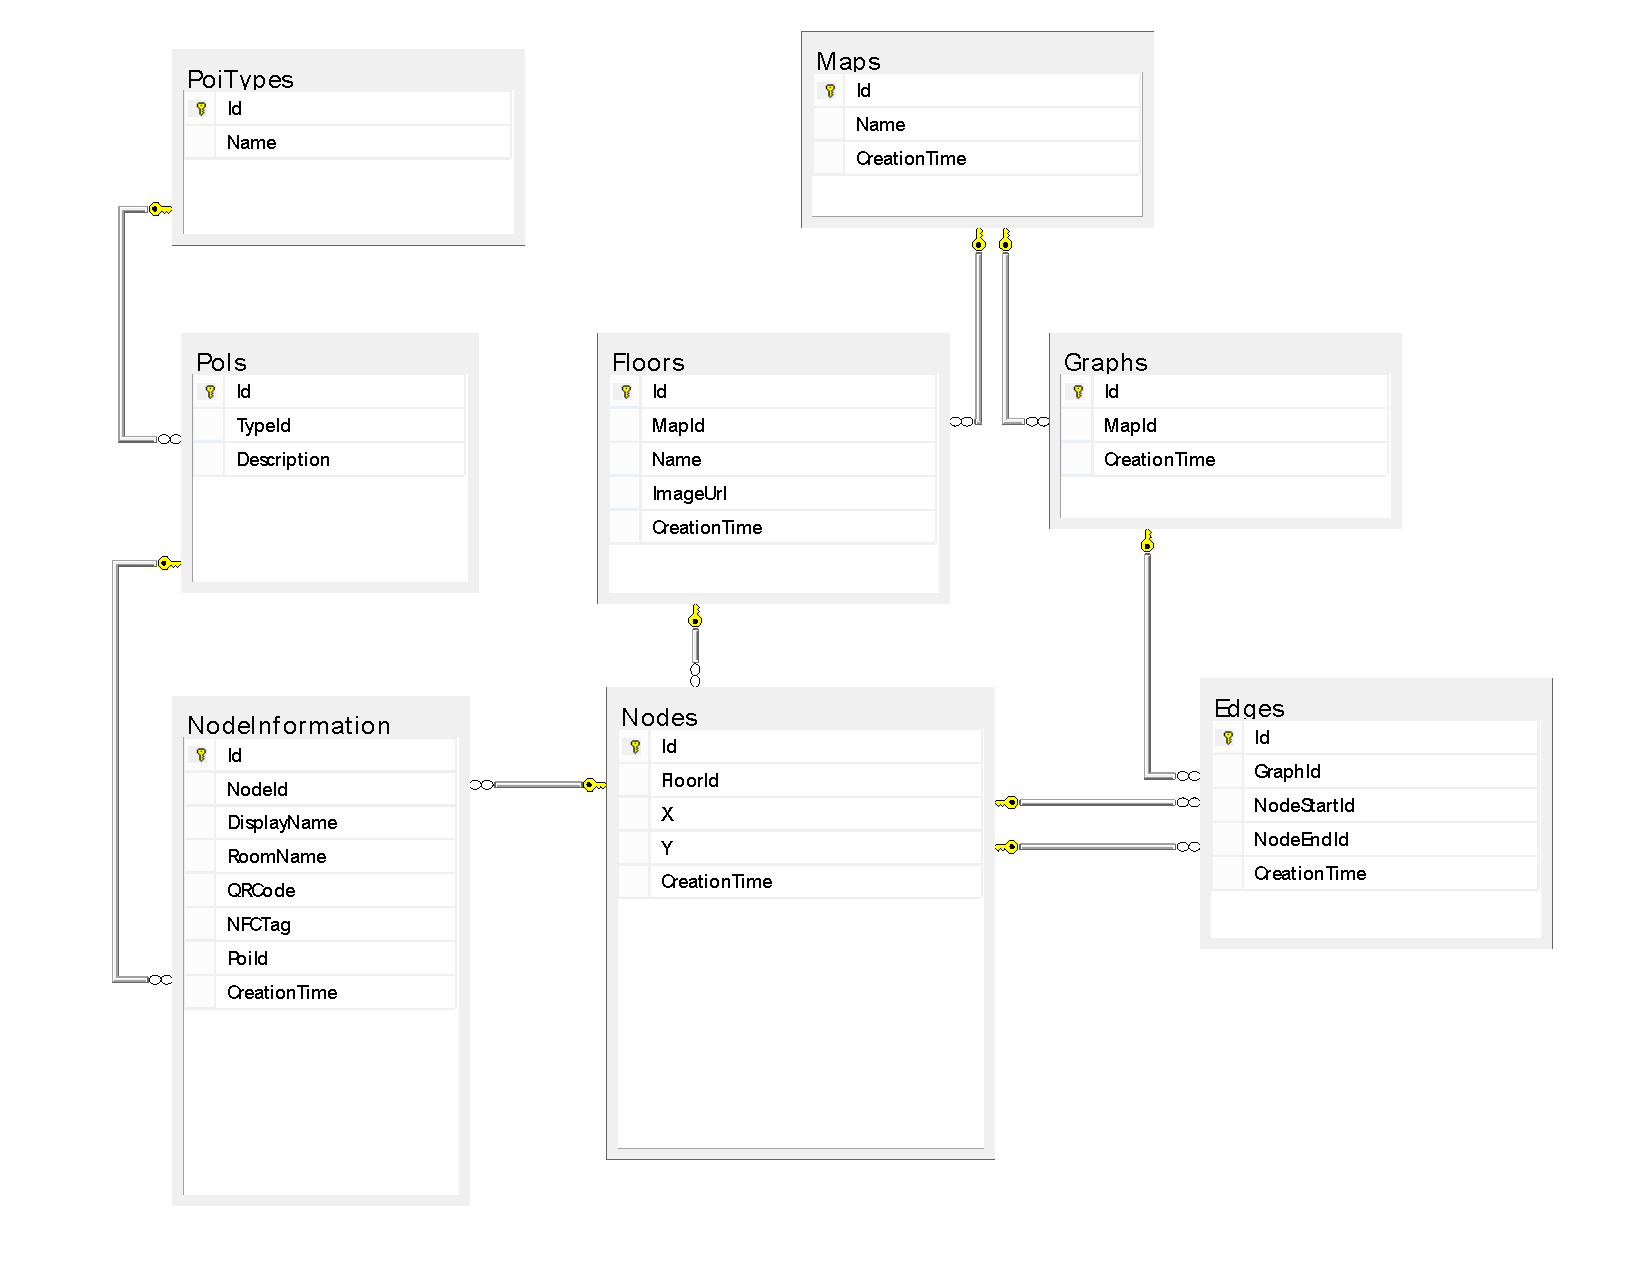
\includegraphics[width=\linewidth]{./Bilder/MapEntities}
\caption{Datenbankmodell f�r die Kartenobjekte}
\label{fig:MapEntities}
\end{figure}

\subsection{Maps}
\label{db:maps:Maps}
F�r jede Karte wird ein Eintrag in dieser Tabelle erzeugt.
Zu jeder Karte wird ein frei vergebener Name und der
Erstellungszeitpunkt gespeichert.

\begin{tabularx}{\textwidth}{|l|l|X|}
\hline \textbf{Spaltenname} & \textbf{Datentyp} & \textbf{Bedeutung}  \\ 
\hline Id 					& INTEGER (PK)		 & ID der Karte \\ 
\hline Name 				& NVARCHAR(255)		 & Name der Karte \\ 
\hline CreationTime 		& DATETIME 			 & Erstellungszeitpunkt\\ 
\hline 
\end{tabularx} 

\subsection{Floors}
F�r jedes Stockwerk wird ein Eintrag in dieser Tabelle angelegt.
Zu jedem Stockwerk wird ein frei vergebener Name, eine URL auf ein
Bild des Stockwerks und ein Erstellungszeitpunkt gespeichert.
Ein Stockwerk ist genau einer Karte zugeordnet.

\begin{tabularx}{\textwidth}{|l|l|X|}
\hline \textbf{Spaltenname} & \textbf{Datentyp} & \textbf{Bedeutung}  \\ 
\hline Id 					& INTEGER (PK)		 & ID des Stockwerks \\
\hline MapId				& INTEGER (FK)		 & ID der zugeordneten Karte \\  
\hline Name 				& NVARCHAR(255)		 & Name des Stockwerks \\ 
\hline ImageUrl				& NVARCHAR(MAX)		 & URL des Bilds \\ 
\hline CreationTime 		& DATETIME 			 & Erstellungszeitpunkt\\ 
\hline 
\end{tabularx} 

\subsection{Graphs}
Ein Graph beschreibt die Knoten- und Kantenstruktur auf einer Karte.
Dazu werden alle Kanten mit dem Graphen verkn�pft. �ber die Kanten
sind auch die Knoten mit dem Graphen indirekt verkn�pft.

\begin{tabularx}{\textwidth}{|l|l|X|}
\hline \textbf{Spaltenname} & \textbf{Datentyp} & \textbf{Bedeutung}  \\ 
\hline Id 					& INTEGER (PK)		 & ID des Graphen \\
\hline MapId				& INTEGER (FK)		 & ID der zugeordneten Karte \\  
\hline CreationTime 		& DATETIME 			 & Erstellungszeitpunkt\\ 
\hline 
\end{tabularx} 

\subsection{Edges}
Eine Kante verkn�pft zwei Knoten in einem Graphen.

\begin{tabularx}{\textwidth}{|l|l|X|}
\hline \textbf{Spaltenname} & \textbf{Datentyp} & \textbf{Bedeutung}  \\ 
\hline Id 					& INTEGER (PK)		 & ID der Kante \\
\hline GraphId				& INTEGER (FK)		 & ID der zugeordneten Graphen \\  
\hline NodeStartId			& INTEGER (FK)		 & ID des Startknotens \\  
\hline NodeEndId			& INTEGER (FK)		 & ID des Endknotens \\  
\hline CreationTime 		& DATETIME 			 & Erstellungszeitpunkt\\ 
\hline 
\end{tabularx} 

\subsection{Nodes}
Die Position eines  Knoten wird durch die Zuordnung zu einem Stockwerk
und seine X/Y-Koordinaten auf diesem Stockwerk bestimmt. Au�erdem wird
der Erstellungszeitpunkt eines Knotens gespeichert.

Die X- und Y-Koordinaten werden im Bereich 0.0 bis 1.0 gespeichert. 
Dabei bedeutet 0.0 ganz links (X) oder ganz oben (Y) und 1.0
ganz rechts (X) bzw. ganz unten (Y) auf dem Bild des Stockwerks.

\begin{tabularx}{\textwidth}{|l|l|X|}
\hline \textbf{Spaltenname} & \textbf{Datentyp} & \textbf{Bedeutung}  \\ 
\hline Id 					& INTEGER (PK)		 & ID der Knotens \\
\hline FloorId				& INTEGER (FK)		 & ID der zugeordneten Stockwerks \\  
\hline X					& DECIMAL(18,17)	 & X-Koordinate auf dem Stockwerk \\  
\hline Y					& DECIMAL(18,17)	 & Y-Koordinate auf dem Stockwerk \\  
\hline CreationTime 		& DATETIME 			 & Erstellungszeitpunkt\\ 
\hline 
\end{tabularx} 

\subsection{NodeInformation}
\label{db:maps:NodeInfo}
Zu einem Knoten k�nnen noch weitere Informationen hinterlegt werden.
Diese sind optional und werden nur zu wichtigen Knoten wie
Seminarr�umen, B�ros und Toiletten hinzugef�gt. �ber die Knoteninformationen
kann auch ein PoI mit dem Knoten verkn�pft werden.

\begin{tabularx}{\textwidth}{|l|l|X|}
\hline \textbf{Spaltenname} & \textbf{Datentyp} & \textbf{Bedeutung}  \\ 
\hline Id 					& INTEGER (PK)		 & ID der Knoteninformation \\
\hline NodeId				& INTEGER (FK)		 & ID der zugeordneten Knotens \\  
\hline DisplayName			& NVARCHAR(50)		 & Name der angezeigt werden soll \\  
\hline RoomName				& NVARCHAR(255)		 & Offizieller Raumname (z.B. B4.0.1.11) \\  
\hline QRCode				& NVARCHAR(255)		 & Hinterlegter QR-Code \\ 
\hline NFCTAG				& NVARCHAR(50)		 & Hinterlegtes NFC-Tag \\ 
\hline PoiId				& INTEGER (FK)		 & Optionaler zugeordneter PoI \\ 
\hline CreationTime 		& DATETIME 			 & Erstellungszeitpunkt\\ 
\hline 
\end{tabularx} 

\subsection{PoIs}
\label{db:maps:PoIs}
Ein PoI (Point of Interest) kategorisiert f�r den Benutzer relevante Knoten.
Hier kann z.B. nach Dozentenb�ros, Mensa, Bibliothek und Toiletten gefiltert
werden.

\begin{tabularx}{\textwidth}{|l|l|X|}
\hline \textbf{Spaltenname} & \textbf{Datentyp} & \textbf{Bedeutung}  \\ 
\hline Id 					& INTEGER (PK)		 & ID des Knotens \\
\hline TypeId				& INTEGER (FK)		 & ID des PoI-Typs \\  
\hline Description			& NVARCHAR(MAX)		 & Zus�tzliche Beschreibung des PoIs \\  
\hline 
\end{tabularx} 

\subsection{PoiTypes}
Diese Tabelle enth�lt die m�glichen Typen von PoIs.

\begin{tabularx}{\textwidth}{|l|l|X|}
\hline \textbf{Spaltenname} & \textbf{Datentyp} & \textbf{Bedeutung}  \\ 
\hline Id 					& INTEGER (PK)		 & ID des PoI-Typs \\
\hline Name					& NVARCHAR(255)		 & Name des PoI-Typs \\  
\hline 
\end{tabularx} 
\section{Users}
\label{sec:Users}

\begin{figure}[H]
\centering
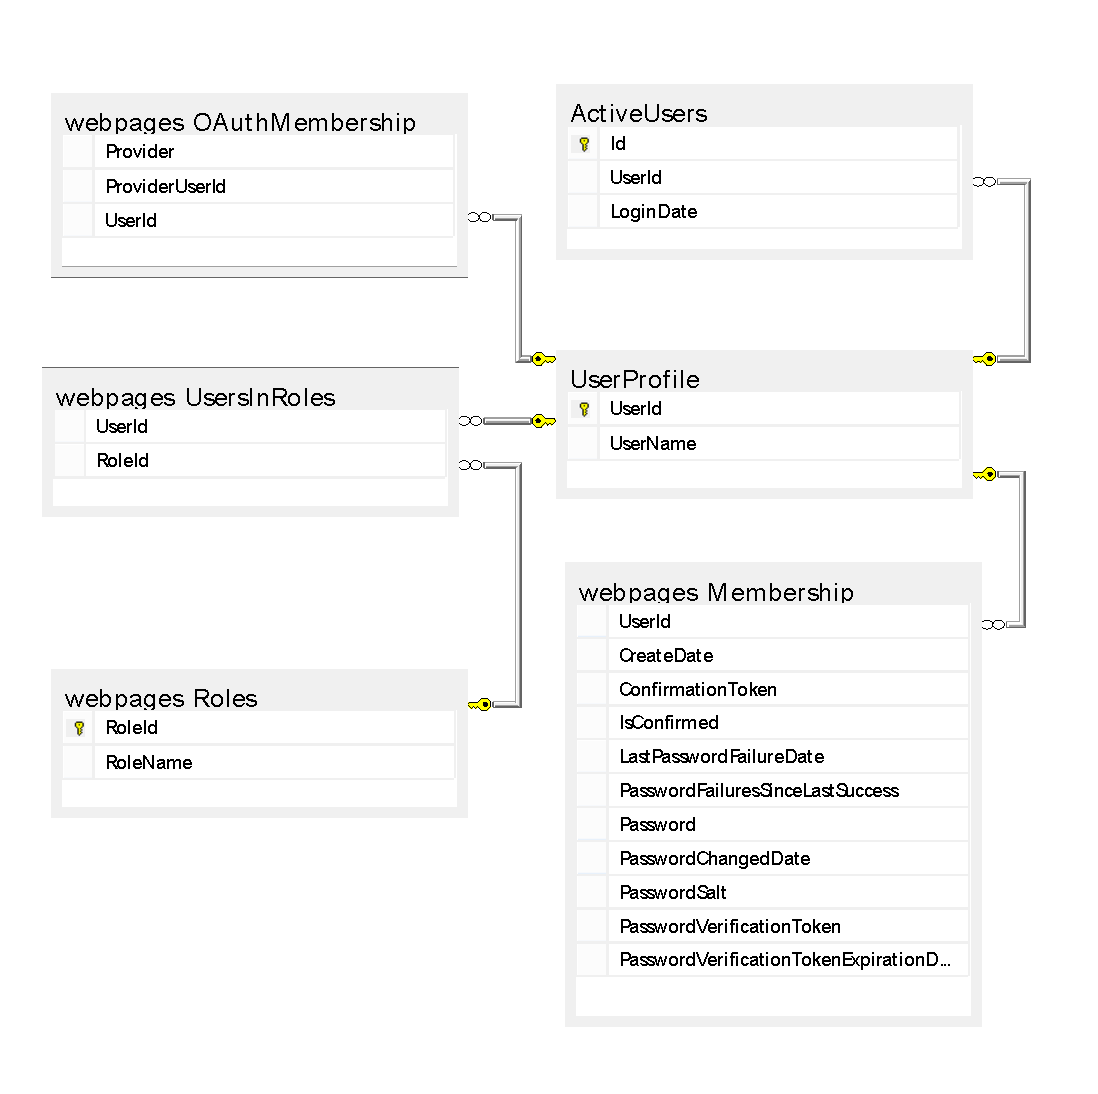
\includegraphics[width=1.0\linewidth]{./Bilder/UserEntities}
\caption{Datenbankmodell f�r Benutzerobjekte}
\label{fig:UserEntities}
\end{figure}

\subsection{MVC spezifische Tabellen}
Alle Tabellen aus dem Diagramm \ref{fig:UserEntities} mit Ausnahme der
ActiveUsers-Tabelle werden von MVC generiert und verwaltet. Sie dienen zur Benutzerauthentifizierung und zur Autorisierung. 

Relevant f�r StudMap sind die Tabellen "'webpages\_Roles"' und
"'webpages\_UserInRoles"'. Hier werden bestehenden Nutzern Rollen
zugewiesen. Um die Admin-Oberfl�che nutzen zu k�nnen, muss einem
Nutzer die Rolle "'Admin"' zugewiesen worden sein.

\subsection{ActiveUsers}
In dieser Tabelle wird festgehalten, welche Benutzer innerhalb 
eines festgelegten Zeitraums unsere App benutzt haben
Diese Tabelle kann z.B. um die letzte Position des Nutzers
erweitert werden. Dadurch k�nnten andere Nutzer sehen, wer 
gerade in ihrer N�he ist.

\begin{tabularx}{\textwidth}{|l|l|X|}
\hline \textbf{Spaltenname} & \textbf{Datentype} & \textbf{Bedeutung}  \\ 
\hline Id 					& INTEGER (PK)		 & ID des Eintrags \\ 
\hline UserId 				& INTEGER (FK)		 & ID des Nutzers \\ 
\hline LoginDate 	     	& DATETIME 			 & Zeitpunkt der letzten Anmeldung bzw. Nutzung der App\\ 
\hline 
\end{tabularx} 


% TODOS:
% - Datenbankmodell �berarbeiten
% - Stored Procedures
% - Views